\documentclass[]{article}
\usepackage{lmodern}
\usepackage{amssymb,amsmath}
\usepackage{ifxetex,ifluatex}
\usepackage{fixltx2e} % provides \textsubscript
\ifnum 0\ifxetex 1\fi\ifluatex 1\fi=0 % if pdftex
  \usepackage[T1]{fontenc}
  \usepackage[utf8]{inputenc}
\else % if luatex or xelatex
  \ifxetex
    \usepackage{mathspec}
  \else
    \usepackage{fontspec}
  \fi
  \defaultfontfeatures{Ligatures=TeX,Scale=MatchLowercase}
\fi
% use upquote if available, for straight quotes in verbatim environments
\IfFileExists{upquote.sty}{\usepackage{upquote}}{}
% use microtype if available
\IfFileExists{microtype.sty}{%
\usepackage{microtype}
\UseMicrotypeSet[protrusion]{basicmath} % disable protrusion for tt fonts
}{}
\usepackage[margin=1in]{geometry}
\usepackage{hyperref}
\hypersetup{unicode=true,
            pdftitle={Authorship Agreement},
            pdfborder={0 0 0},
            breaklinks=true}
\urlstyle{same}  % don't use monospace font for urls
\usepackage{graphicx,grffile}
\makeatletter
\def\maxwidth{\ifdim\Gin@nat@width>\linewidth\linewidth\else\Gin@nat@width\fi}
\def\maxheight{\ifdim\Gin@nat@height>\textheight\textheight\else\Gin@nat@height\fi}
\makeatother
% Scale images if necessary, so that they will not overflow the page
% margins by default, and it is still possible to overwrite the defaults
% using explicit options in \includegraphics[width, height, ...]{}
\setkeys{Gin}{width=\maxwidth,height=\maxheight,keepaspectratio}
\IfFileExists{parskip.sty}{%
\usepackage{parskip}
}{% else
\setlength{\parindent}{0pt}
\setlength{\parskip}{6pt plus 2pt minus 1pt}
}
\setlength{\emergencystretch}{3em}  % prevent overfull lines
\providecommand{\tightlist}{%
  \setlength{\itemsep}{0pt}\setlength{\parskip}{0pt}}
\setcounter{secnumdepth}{0}
% Redefines (sub)paragraphs to behave more like sections
\ifx\paragraph\undefined\else
\let\oldparagraph\paragraph
\renewcommand{\paragraph}[1]{\oldparagraph{#1}\mbox{}}
\fi
\ifx\subparagraph\undefined\else
\let\oldsubparagraph\subparagraph
\renewcommand{\subparagraph}[1]{\oldsubparagraph{#1}\mbox{}}
\fi

%%% Use protect on footnotes to avoid problems with footnotes in titles
\let\rmarkdownfootnote\footnote%
\def\footnote{\protect\rmarkdownfootnote}

%%% Change title format to be more compact
\usepackage{titling}

% Create subtitle command for use in maketitle
\newcommand{\subtitle}[1]{
  \posttitle{
    \begin{center}\large#1\end{center}
    }
}

\setlength{\droptitle}{-2em}

  \title{Authorship Agreement}
    \pretitle{\vspace{\droptitle}\centering\huge}
  \posttitle{\par}
    \author{}
    \preauthor{}\postauthor{}
    \date{}
    \predate{}\postdate{}
  

\begin{document}
\maketitle

\hypertarget{guidelines-for-authorship1}{%
\section{Guidelines for Authorship1}\label{guidelines-for-authorship1}}

1Adapted from the Saltmarsh Habitat \& Avian Research Program
(\url{https://www.tidalmarshbirds.org/}) Guidelines for Authorship
Standard Operating Procedure.

Download as PDF

\textbf{Table of Contents:}

\begin{enumerate}
\def\labelenumi{\arabic{enumi}.}
\item
  \protect\hyperlink{author}{\textbf{Authorship Criteria}}

  \begin{itemize}
  \item
    \protect\hyperlink{threshold}{\emph{Consider Thresholds of Effort}}
  \item
    \protect\hyperlink{involvement}{\emph{Offer Further Involvement}}
  \item
    \protect\hyperlink{inclusion}{\emph{Use Inclusion to Deal with
    Uncertainty}}
  \item
    \protect\hyperlink{alum}{\emph{Invite Alumni to Participate when
    Appropriate}}
  \end{itemize}
\item
  \protect\hyperlink{order}{\textbf{Author Order and Etiquette}}
\item
  \protect\hyperlink{doc}{\textbf{A Living Document}}
\item
  \protect\hyperlink{duty}{\textbf{Duty as a co-author}}
\end{enumerate}

\begin{center}\rule{0.5\linewidth}{\linethickness}\end{center}

Deciding authorship on scientific publications can be complicated
because practices and cultural norms vary across disciplines and even
across labs within the same discipline. This is especially relevant in
ecology, where standardized guidelines are lacking and a diversity of
options exist for deciding authorship and author order. These guidelines
outline a set of criteria for authorship determinations. These criteria
are presented as guidelines, because a common set of expectations is
important to maintain mutual satisfaction among co- authors. We
recognize, however, that some flexibility will be required and
communication is essential to the process. Before all else, remember
\textbf{conversations regarding authorship for each manuscript should
happen early, frequently, openly, and inclusively}. A conversation
should be expected when the paper is first conceived and should be
revisited periodically as each project develops.

\hypertarget{authorship-criteria}{%
\subsection{\texorpdfstring{\textbf{Authorship
Criteria}}{Authorship Criteria}}\label{authorship-criteria}}

Authorship on a manuscript is warranted when a researcher has made a
substantial contribution to the manuscript in question (not the overall
project as a whole), as defined by any \textbf{two} of the following:

\begin{itemize}
\item
  Conceiving of ideas and/or study design and/or analytical approach
\item
  Writing of the manuscript (or sections)
\item
  Reviewing and editing the manuscript
\item
  Analyzing data
\item
  Interpreting results
\item
  Collecting data in field or lab (except in rare circumstances this
  will not include temporary technicians)
\item
  Creating or managing critical databases (e.g.~demographic database,
  historical abundance estimates spreadsheet)
\item
  Obtaining funding (e.g., proposal writing, grant management, and
  project reports)
\end{itemize}

Other things are important to keep in mind (expanded upon in the
sections below).

\begin{itemize}
\item
  \emph{A conversation is necessary for each manuscript}
\item
  \emph{Consider thresholds of effort (``could the study have been done
  without the contribution?'')}
\item
  \emph{Offer further involvement}
\item
  \emph{Use inclusion to deal with uncertainty (``better to be inclusive
  than to exclude'')}
\item
  \emph{Primary authors and their advisors/PIs/mentors will make the
  final decision on authorship}
\item
  \emph{Invite prior individuals (alumni) to participate when
  appropriate}
\item
  \emph{There are exceptions for grant deliverables.}
\item
  \textbf{\emph{When in doubt, talk it out!}}
\end{itemize}

\emph{Consider Thresholds of Effort}

Ultimately, the primary author must have some leeway in making
authorship decisions, and ensuring that a certain minimum threshold of
contribution has been made. When the level of the contribution to the
particular manuscript is unclear (e.g.~as in the case of data
collection), the deciding question becomes ``could the study have been
done without that person's contribution?''

For instance, did the extra work amount to a few data points within a
huge dataset (if the analysis was enhanced by their participation, but
was possible without it, authorship may not be warranted), or were the
data points critical to establishing the pattern (if the analysis is
impossible without the data from this study site, or if trends depend on
those data, authorship is more clearly warranted). Other considerations:
If a researcher is collecting data for a study that is not their own,
did they do extra work that they would not otherwise have done on their
own study site or for their own study (if so, the case for authorship
increases)? Did the effort amount to a few days of fieldwork (may not
warrant authorship) or a season's worth of logistics and data collection
(more clearly warrants authorship)?

\emph{Offer Further Involvement}

In some instances, a contributor may have clearly passed a threshold of
effort (see previous), but will have only contributed to one of the
categories that would qualify them for consideration of authorship. In
these instances, it is the primary author's responsibility to reach out
to the contributor early in the writing process and have a conversation
about further involvement. The second category can be easily achieved by
assistance with developing and reviewing the manuscript, and
contributors that have clearly passed a threshold of effort should be
given that opportunity.

\emph{Use Inclusion to Deal with Uncertainty}

Recognize that the contribution of effort is a gradient with clear
endpoints (one data point out of two probably gets you authorship, one
data point out of 1,000 probably doesn't), so there will likely be
situations where it is unclear (200 data points out of 1,000?). If there
is any uncertainty in gauging the contribution, it is better to be
inclusive than to exclude, and it is better to talk directly to the
contributor explicitly. A quick phone call made in a spirit of inclusion
can almost always improve the situation for everyone, both for this
manuscript and for future collaboration.

\emph{Invite Alumni to Participate when Appropriate}

As data collected by others who have moved on are used in analysis, we
need to give them credit for their prior work. If the data have already
been published in another form and their papers can be cited, this may
be enough. Authorship may be warranted or offered, however, under
several circumstances. First, if the individual was involved in the
conception of the ideas in the new manuscript, this would warrant their
inclusion. Second, if the new manuscript is based largely on the data
(or conceptual groundwork) of a single individual (similar to the rules
for contemporary contributors, could the analysis be completed without
their data?), authorship should be considered. If the previous work of
prior individuals passes the Threshold of Effort test for any reason,
the burden is on the PI involved to offer the opportunity for further
engagement in the new manuscript to new individuals, preferably early in
the process. If prior individuals respond positively and stay involved,
then they should be authors on the new work. Prior individuals are
responsible for deciding to stay engaged and following through with
their involvement. Importantly, prior individuals should understand that
if they do not respond to inquiries about authorship, historical
datasets can still be used, but they will not be included as authors.
This same approach may be followed for the advisors of prior individuals
if they pass the Threshold.

\hypertarget{author-order-and-etiquette}{%
\subsection{\texorpdfstring{\textbf{Author Order and
Etiquette}}{Author Order and Etiquette}}\label{author-order-and-etiquette}}

The order of authors on publications will follow the practice of
first-last author emphasis. The first author will be the person who did
the majority of the work, carried out the study, and will often be a the
primary writer of the manuscript. Typically, the last author should be
the lab PI. ``Credit'' or ``importance'' is attributed to authors in the
following order: first, last, 2nd, 3rd, 4th, etc. Final decisions
regarding author order ultimately lie with the first author, in
consultation with their advisor, PI or mentor. Authors that disagree
with the draft author order, however, should feel comfortable voicing
their concerns. More importantly, primary authors should ask
specifically for co-authors to approve the final order via email.

Anyone listed as an author must be given a fair opportunity to read and
comment on the manuscript. If prospective authors do not respond in a
reasonable amount of time, they should be removed, barring exceptional
circumstances (the response could be as simple as ``manuscript is good
to go'', as long as the author acknowledges and approves the content).
The lead author should give AT LEAST two weeks for the response period
and should specify a date by which comments are due. Two corollaries of
this guideline are 1) anyone has the right to request removal as author
from a paper for any reason, including a personal judgment of failure to
cross the Threshold for Effort, and 2) no one should ever be an author
on a manuscript where they did not approve the final submitted draft
(note that many journals have this requirement).

It is the primary author's responsibility, as corresponding author, to
provide all co-authors with:

\begin{itemize}
\item
  A digital version of the final submitted draft
\item
  News of all significant correspondence with the editor/publisher
\item
  The opportunity to assist with revisions
\item
  A digital version of all revisions submitted for publication and the
  responses to reviewers
\item
  Page proofs and the opportunity to comment on them
\item
  A final pdf of all published papers
\end{itemize}

\hypertarget{a-living-document}{%
\subsection{\texorpdfstring{\textbf{A Living
Document}}{A Living Document}}\label{a-living-document}}

Expectations for authorship are a set of evolving cultural norms. This
means that 1) they must be taught anew to each set of students and/or
new individual early in their involvement with the project and 2) the
guidelines in this document need to be revisited and updated regularly
(\textasciitilde{}annually or as needed).

\begin{center}\rule{0.5\linewidth}{\linethickness}\end{center}

\hypertarget{duty-as-a-co-author}{%
\subsection{\texorpdfstring{\textbf{Duty as a
co-author}}{Duty as a co-author}}\label{duty-as-a-co-author}}

The dissemination of research to the broader scientific community is not
only part of the research process, but perhaps the ultimate reason for
conducting research in the first place. There is an expectation and
responsiblity to share one's work with the broader community (Cooke et
al.~2014). It goes without saying that composing a manuscript by
committee can be difficult. Co-authorship comes about in a variety of
ways some of which may not require a formal role in writting but rather
the collection of data, editing of the manuscript, etc. Some manuscripts
are planned in advanced and have the luxuary of identfying the core
author pool. Other manuscripts are produced \emph{ad-hoc}. Regardless of
the origin it is recommended that if the mansucript has more than two
authors it is advisable that a lead author along with a supporting
person (typically senior author assumes this role) be identified. The
objective of having two (or more) authors is to have these individuals
generate a paper that is as close to final as possible, after all
\emph{two-eyes are better than one}. Letting other co-authors know that
the paper is ready to move forward in the eyes of both the lead senior
authors will often help to elicit a rapid review and response by
co-authors.

Everyone is busy, therefore some degree of time-management is needed
when composing an manuscript. Therefore it is recommended that tentative
deadlines/time-periods are discussed early and often. If necessary these
deadline can be revised as needed due to changing priorties within
reason but make sure these changes are communicated amongst all authors.
Once a draft manuscript is produced and ready for co-author input
provide a reasonable review deadline (couple of weeks).
\emph{Typically}, if co-authors are unresponsive its not they don't find
the manuscript important. It is possible that it has been shuffled down
the dreded \emph{``to do''} list or they just forgot. This has happended
to all of us at some point. Therefore a simple reminder would be helpful
to re-engague the co-authors. Below is a flow chart from Cooke et al.
(2014) with a suggested example of sequence of events to work with tardy
or non-responsive co-authors.

\begin{figure}

{\centering 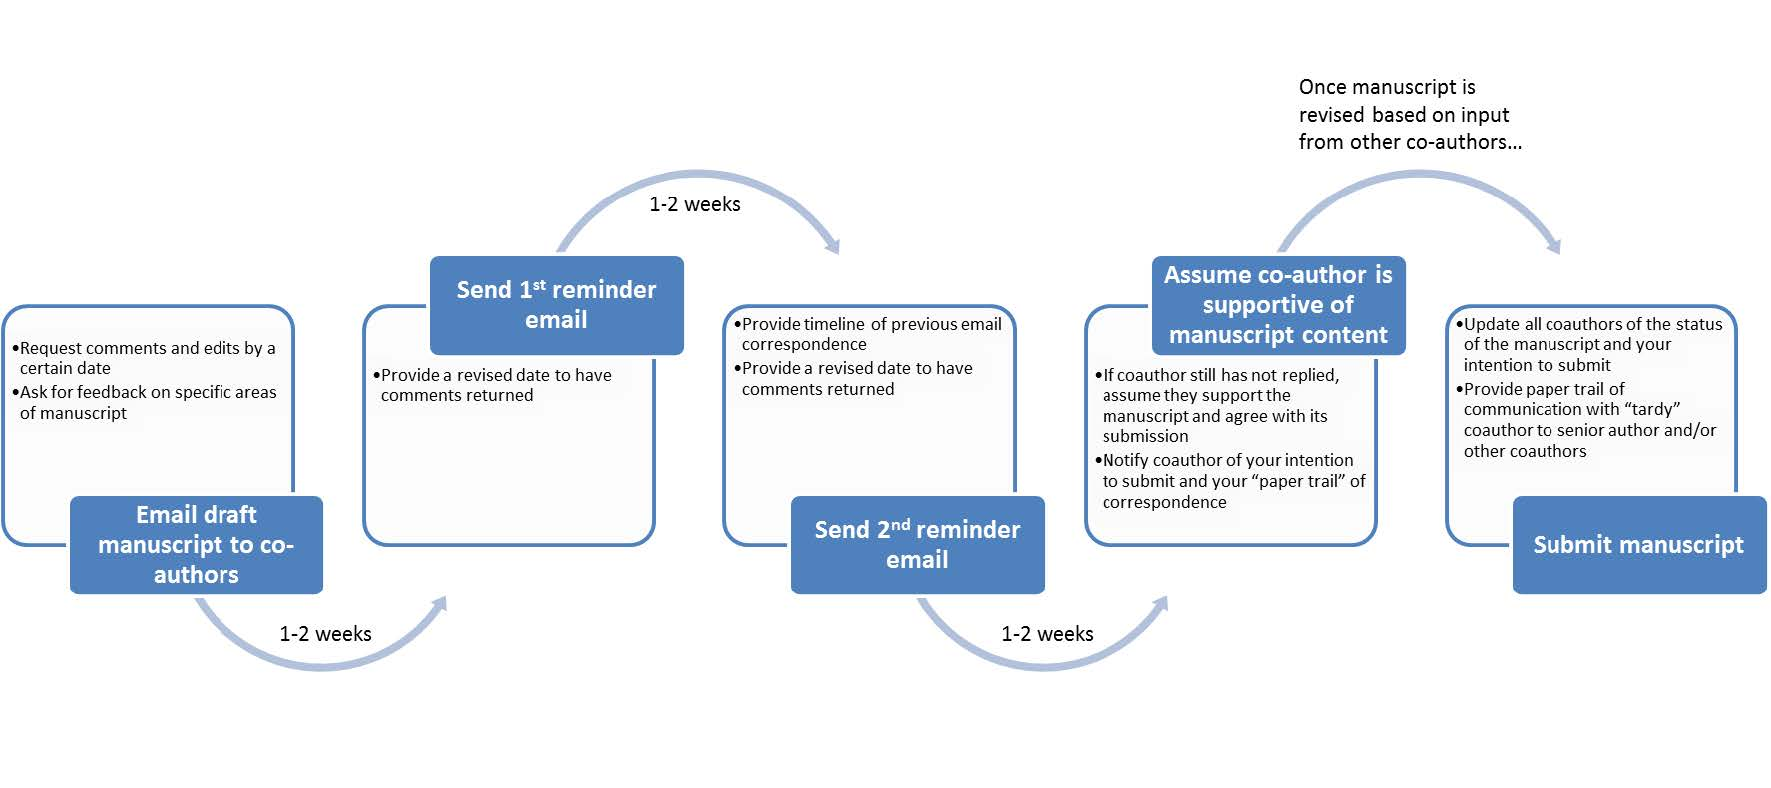
\includegraphics[width=0.7\linewidth]{../images/Cooke et al_Fig1} 

}

\caption{Flow-diagram with a possile sequence of events for working with tardy or non-responsive co-authors when preparing a manuscript for submission to a journal. From Cooke et al. (2014).}\label{fig:unnamed-chunk-2}
\end{figure}

As suggested above, if co-authors are completely unresponsive it is the
lead authors progrative, with input from co-authors to remove
unresponsice co-authors. The Committee on Publication Ethics
(\href{https://publicationethics.org/authorship}{COPE}), has additional
guideance information regarding authorship and ethics.

\hypertarget{reference}{%
\subsection{Reference}\label{reference}}

\begin{itemize}
\item
  Cooke SJ, Donaldson MR, Clark TD (2014) Practical guidance for early
  career researchers dealing with tardy or unresponsive co-authors.
  Ideas in Ecology and Evolution. 1(7).
  \href{https://ojs.library.queensu.ca/index.php/IEE/article/view/5484}{Link}
\item
  Saltmarsh Habitat \& Avian Research Program (2014) Guidelines for
  authorship. Saltmarsh Habitat \& Avian Research Program.
  \url{https://www.tidalmarshbirds.org/}.
\end{itemize}


\end{document}
